\section{Estrutura da Rede Neural Artificial}

\begin{frame}{Estrutura da PIRNN utilizada}
  A PIRNN utilizada consiste em 4 camadas, todas com a função de ativação tangente hiperbólica $(\sigma)$, com exceção da saída, que não possui função de ativação.

  No total, a rede possui $32+32+32+2=98$ neurônios.

  \begin{figure}
    \centering
    \resizebox{0.45\textwidth}{!}{% Graphic for TeX using PGF
% Title: /home/silas/Downloads/prh-35.1/LaTeX/common/figures/pirnn-diagram.dia
% Creator: Dia v0.97+git
% CreationDate: Tue May 20 14:37:33 2025
% For: silas
% \usepackage{tikz}
% The following commands are not supported in PSTricks at present
% We define them conditionally, so when they are implemented,
% this pgf file will use them.
\ifx\du\undefined
  \newlength{\du}
\fi
\setlength{\du}{15\unitlength}
\begin{tikzpicture}[even odd rule]
  \pgftransformxscale{1.000000}
  \pgftransformyscale{-1.000000}
  \definecolor{dialinecolor}{rgb}{0.000000, 0.000000, 0.000000}
  \pgfsetstrokecolor{dialinecolor}
  \pgfsetstrokeopacity{1.000000}
  \definecolor{diafillcolor}{rgb}{1.000000, 1.000000, 1.000000}
  \pgfsetfillcolor{diafillcolor}
  \pgfsetfillopacity{1.000000}
  \pgfsetlinewidth{0.100000\du}
  \pgfsetdash{}{0pt}
  \pgfsetmiterjoin
  \definecolor{diafillcolor}{rgb}{1.000000, 1.000000, 1.000000}
  \pgfsetfillcolor{diafillcolor}
  \pgfsetfillopacity{1.000000}
  \pgfpathellipse{\pgfpoint{29.000000\du}{16.000000\du}}{\pgfpoint{1.000000\du}{0\du}}{\pgfpoint{0\du}{1.000000\du}}
  \pgfusepath{fill}
  \definecolor{dialinecolor}{rgb}{0.000000, 0.000000, 0.000000}
  \pgfsetstrokecolor{dialinecolor}
  \pgfsetstrokeopacity{1.000000}
  \pgfpathellipse{\pgfpoint{29.000000\du}{16.000000\du}}{\pgfpoint{1.000000\du}{0\du}}{\pgfpoint{0\du}{1.000000\du}}
  \pgfusepath{stroke}
  % setfont left to latex
  \definecolor{dialinecolor}{rgb}{0.000000, 0.000000, 0.000000}
  \pgfsetstrokecolor{dialinecolor}
  \pgfsetstrokeopacity{1.000000}
  \definecolor{diafillcolor}{rgb}{0.000000, 0.000000, 0.000000}
  \pgfsetfillcolor{diafillcolor}
  \pgfsetfillopacity{1.000000}
  \node[anchor=base,inner sep=0pt, outer sep=0pt,color=dialinecolor] at (29.000000\du,16.194063\du){};
  \pgfsetlinewidth{0.100000\du}
  \pgfsetdash{}{0pt}
  \pgfsetmiterjoin
  \definecolor{diafillcolor}{rgb}{1.000000, 1.000000, 1.000000}
  \pgfsetfillcolor{diafillcolor}
  \pgfsetfillopacity{1.000000}
  \pgfpathellipse{\pgfpoint{33.000000\du}{18.000000\du}}{\pgfpoint{1.000000\du}{0\du}}{\pgfpoint{0\du}{1.000000\du}}
  \pgfusepath{fill}
  \definecolor{dialinecolor}{rgb}{0.000000, 0.000000, 0.000000}
  \pgfsetstrokecolor{dialinecolor}
  \pgfsetstrokeopacity{1.000000}
  \pgfpathellipse{\pgfpoint{33.000000\du}{18.000000\du}}{\pgfpoint{1.000000\du}{0\du}}{\pgfpoint{0\du}{1.000000\du}}
  \pgfusepath{stroke}
  % setfont left to latex
  \definecolor{dialinecolor}{rgb}{0.000000, 0.000000, 0.000000}
  \pgfsetstrokecolor{dialinecolor}
  \pgfsetstrokeopacity{1.000000}
  \definecolor{diafillcolor}{rgb}{0.000000, 0.000000, 0.000000}
  \pgfsetfillcolor{diafillcolor}
  \pgfsetfillopacity{1.000000}
  \node[anchor=base,inner sep=0pt, outer sep=0pt,color=dialinecolor] at (33.000000\du,18.194063\du){};
  \pgfsetlinewidth{0.100000\du}
  \pgfsetdash{}{0pt}
  \pgfsetmiterjoin
  \definecolor{diafillcolor}{rgb}{1.000000, 1.000000, 1.000000}
  \pgfsetfillcolor{diafillcolor}
  \pgfsetfillopacity{1.000000}
  \pgfpathellipse{\pgfpoint{33.000000\du}{23.000000\du}}{\pgfpoint{1.000000\du}{0\du}}{\pgfpoint{0\du}{1.000000\du}}
  \pgfusepath{fill}
  \definecolor{dialinecolor}{rgb}{0.000000, 0.000000, 0.000000}
  \pgfsetstrokecolor{dialinecolor}
  \pgfsetstrokeopacity{1.000000}
  \pgfpathellipse{\pgfpoint{33.000000\du}{23.000000\du}}{\pgfpoint{1.000000\du}{0\du}}{\pgfpoint{0\du}{1.000000\du}}
  \pgfusepath{stroke}
  % setfont left to latex
  \definecolor{dialinecolor}{rgb}{0.000000, 0.000000, 0.000000}
  \pgfsetstrokecolor{dialinecolor}
  \pgfsetstrokeopacity{1.000000}
  \definecolor{diafillcolor}{rgb}{0.000000, 0.000000, 0.000000}
  \pgfsetfillcolor{diafillcolor}
  \pgfsetfillopacity{1.000000}
  \node[anchor=base,inner sep=0pt, outer sep=0pt,color=dialinecolor] at (33.000000\du,23.194063\du){};
  % setfont left to latex
  \definecolor{dialinecolor}{rgb}{0.000000, 0.000000, 0.000000}
  \pgfsetstrokecolor{dialinecolor}
  \pgfsetstrokeopacity{1.000000}
  \definecolor{diafillcolor}{rgb}{0.000000, 0.000000, 0.000000}
  \pgfsetfillcolor{diafillcolor}
  \pgfsetfillopacity{1.000000}
  \node[anchor=base,inner sep=0pt, outer sep=0pt,color=dialinecolor] at (33.000000\du,18.221562\du){$h_1^{(t)}$};
  % setfont left to latex
  \definecolor{dialinecolor}{rgb}{0.000000, 0.000000, 0.000000}
  \pgfsetstrokecolor{dialinecolor}
  \pgfsetstrokeopacity{1.000000}
  \definecolor{diafillcolor}{rgb}{0.000000, 0.000000, 0.000000}
  \pgfsetfillcolor{diafillcolor}
  \pgfsetfillopacity{1.000000}
  \node[anchor=base,inner sep=0pt, outer sep=0pt,color=dialinecolor] at (33.000000\du,23.221562\du){$h_2^{(t)}$};
  % setfont left to latex
  \definecolor{dialinecolor}{rgb}{0.000000, 0.000000, 0.000000}
  \pgfsetstrokecolor{dialinecolor}
  \pgfsetstrokeopacity{1.000000}
  \definecolor{diafillcolor}{rgb}{0.000000, 0.000000, 0.000000}
  \pgfsetfillcolor{diafillcolor}
  \pgfsetfillopacity{1.000000}
  \node[anchor=base west,inner sep=0pt,outer sep=0pt,color=dialinecolor] at (33.000000\du,18.000000\du){};
  \pgfsetlinewidth{0.100000\du}
  \pgfsetdash{}{0pt}
  \pgfsetmiterjoin
  {\pgfsetcornersarced{\pgfpoint{1.000000\du}{1.000000\du}}\definecolor{diafillcolor}{rgb}{1.000000, 1.000000, 1.000000}
    \pgfsetfillcolor{diafillcolor}
    \pgfsetfillopacity{1.000000}
    \fill (12.500000\du,15.500000\du)--(12.500000\du,17.500000\du)--(17.500000\du,17.500000\du)--(17.500000\du,15.500000\du)--cycle;
  }{\pgfsetcornersarced{\pgfpoint{1.000000\du}{1.000000\du}}\definecolor{dialinecolor}{rgb}{0.000000, 0.000000, 0.000000}
    \pgfsetstrokecolor{dialinecolor}
    \pgfsetstrokeopacity{1.000000}
    \draw (12.500000\du,15.500000\du)--(12.500000\du,17.500000\du)--(17.500000\du,17.500000\du)--(17.500000\du,15.500000\du)--cycle;
  }% setfont left to latex
  \definecolor{dialinecolor}{rgb}{0.000000, 0.000000, 0.000000}
  \pgfsetstrokecolor{dialinecolor}
  \pgfsetstrokeopacity{1.000000}
  \definecolor{diafillcolor}{rgb}{0.000000, 0.000000, 0.000000}
  \pgfsetfillcolor{diafillcolor}
  \pgfsetfillopacity{1.000000}
  \node[anchor=base,inner sep=0pt, outer sep=0pt,color=dialinecolor] at (15.000000\du,16.694063\du){};
  % setfont left to latex
  \definecolor{dialinecolor}{rgb}{0.000000, 0.000000, 0.000000}
  \pgfsetstrokecolor{dialinecolor}
  \pgfsetstrokeopacity{1.000000}
  \definecolor{diafillcolor}{rgb}{0.000000, 0.000000, 0.000000}
  \pgfsetfillcolor{diafillcolor}
  \pgfsetfillopacity{1.000000}
  \node[anchor=base,inner sep=0pt, outer sep=0pt,color=dialinecolor] at (15.000000\du,16.721562\du){$[h_1^{(t-2)}, h_1^{(t-1)}]$};
  \pgfsetlinewidth{0.100000\du}
  \pgfsetdash{}{0pt}
  \pgfsetmiterjoin
  {\pgfsetcornersarced{\pgfpoint{1.000000\du}{1.000000\du}}\definecolor{diafillcolor}{rgb}{1.000000, 1.000000, 1.000000}
    \pgfsetfillcolor{diafillcolor}
    \pgfsetfillopacity{1.000000}
    \fill (12.500000\du,19.500000\du)--(12.500000\du,21.500000\du)--(17.500000\du,21.500000\du)--(17.500000\du,19.500000\du)--cycle;
  }{\pgfsetcornersarced{\pgfpoint{1.000000\du}{1.000000\du}}\definecolor{dialinecolor}{rgb}{0.000000, 0.000000, 0.000000}
    \pgfsetstrokecolor{dialinecolor}
    \pgfsetstrokeopacity{1.000000}
    \draw (12.500000\du,19.500000\du)--(12.500000\du,21.500000\du)--(17.500000\du,21.500000\du)--(17.500000\du,19.500000\du)--cycle;
  }% setfont left to latex
  \definecolor{dialinecolor}{rgb}{0.000000, 0.000000, 0.000000}
  \pgfsetstrokecolor{dialinecolor}
  \pgfsetstrokeopacity{1.000000}
  \definecolor{diafillcolor}{rgb}{0.000000, 0.000000, 0.000000}
  \pgfsetfillcolor{diafillcolor}
  \pgfsetfillopacity{1.000000}
  \node[anchor=base,inner sep=0pt, outer sep=0pt,color=dialinecolor] at (15.000000\du,20.694063\du){};
  \pgfsetlinewidth{0.100000\du}
  \pgfsetdash{}{0pt}
  \pgfsetmiterjoin
  {\pgfsetcornersarced{\pgfpoint{1.000000\du}{1.000000\du}}\definecolor{diafillcolor}{rgb}{1.000000, 1.000000, 1.000000}
    \pgfsetfillcolor{diafillcolor}
    \pgfsetfillopacity{1.000000}
    \fill (12.500000\du,23.500000\du)--(12.500000\du,25.500000\du)--(17.500000\du,25.500000\du)--(17.500000\du,23.500000\du)--cycle;
  }{\pgfsetcornersarced{\pgfpoint{1.000000\du}{1.000000\du}}\definecolor{dialinecolor}{rgb}{0.000000, 0.000000, 0.000000}
    \pgfsetstrokecolor{dialinecolor}
    \pgfsetstrokeopacity{1.000000}
    \draw (12.500000\du,23.500000\du)--(12.500000\du,25.500000\du)--(17.500000\du,25.500000\du)--(17.500000\du,23.500000\du)--cycle;
  }% setfont left to latex
  \definecolor{dialinecolor}{rgb}{0.000000, 0.000000, 0.000000}
  \pgfsetstrokecolor{dialinecolor}
  \pgfsetstrokeopacity{1.000000}
  \definecolor{diafillcolor}{rgb}{0.000000, 0.000000, 0.000000}
  \pgfsetfillcolor{diafillcolor}
  \pgfsetfillopacity{1.000000}
  \node[anchor=base,inner sep=0pt, outer sep=0pt,color=dialinecolor] at (15.000000\du,24.694063\du){};
  % setfont left to latex
  \definecolor{dialinecolor}{rgb}{0.000000, 0.000000, 0.000000}
  \pgfsetstrokecolor{dialinecolor}
  \pgfsetstrokeopacity{1.000000}
  \definecolor{diafillcolor}{rgb}{0.000000, 0.000000, 0.000000}
  \pgfsetfillcolor{diafillcolor}
  \pgfsetfillopacity{1.000000}
  \node[anchor=base,inner sep=0pt, outer sep=0pt,color=dialinecolor] at (15.000000\du,20.721562\du){$[h_2^{(t-2)}, h_2^{(t-1)}]$};
  % setfont left to latex
  \definecolor{dialinecolor}{rgb}{0.000000, 0.000000, 0.000000}
  \pgfsetstrokecolor{dialinecolor}
  \pgfsetstrokeopacity{1.000000}
  \definecolor{diafillcolor}{rgb}{0.000000, 0.000000, 0.000000}
  \pgfsetfillcolor{diafillcolor}
  \pgfsetfillopacity{1.000000}
  \node[anchor=base,inner sep=0pt, outer sep=0pt,color=dialinecolor] at (15.000000\du,24.721562\du){$[q_{\mathrm{in}}^{(t-2)}, q_{\mathrm{in}}^{(t-1)}]$};
  % setfont left to latex
  \definecolor{dialinecolor}{rgb}{0.000000, 0.000000, 0.000000}
  \pgfsetstrokecolor{dialinecolor}
  \pgfsetstrokeopacity{1.000000}
  \definecolor{diafillcolor}{rgb}{0.000000, 0.000000, 0.000000}
  \pgfsetfillcolor{diafillcolor}
  \pgfsetfillopacity{1.000000}
  \node[anchor=base,inner sep=0pt, outer sep=0pt,color=dialinecolor] at (21.000000\du,27.221562\du){Camada RNN};
  \pgfsetlinewidth{0.100000\du}
  \pgfsetdash{}{0pt}
  \pgfsetmiterjoin
  \definecolor{diafillcolor}{rgb}{1.000000, 1.000000, 1.000000}
  \pgfsetfillcolor{diafillcolor}
  \pgfsetfillopacity{1.000000}
  \pgfpathellipse{\pgfpoint{25.000000\du}{16.000000\du}}{\pgfpoint{1.000000\du}{0\du}}{\pgfpoint{0\du}{1.000000\du}}
  \pgfusepath{fill}
  \definecolor{dialinecolor}{rgb}{0.000000, 0.000000, 0.000000}
  \pgfsetstrokecolor{dialinecolor}
  \pgfsetstrokeopacity{1.000000}
  \pgfpathellipse{\pgfpoint{25.000000\du}{16.000000\du}}{\pgfpoint{1.000000\du}{0\du}}{\pgfpoint{0\du}{1.000000\du}}
  \pgfusepath{stroke}
  % setfont left to latex
  \definecolor{dialinecolor}{rgb}{0.000000, 0.000000, 0.000000}
  \pgfsetstrokecolor{dialinecolor}
  \pgfsetstrokeopacity{1.000000}
  \definecolor{diafillcolor}{rgb}{0.000000, 0.000000, 0.000000}
  \pgfsetfillcolor{diafillcolor}
  \pgfsetfillopacity{1.000000}
  \node[anchor=base,inner sep=0pt, outer sep=0pt,color=dialinecolor] at (25.000000\du,16.194063\du){};
  \pgfsetlinewidth{0.100000\du}
  \pgfsetdash{}{0pt}
  \pgfsetmiterjoin
  \definecolor{diafillcolor}{rgb}{1.000000, 1.000000, 1.000000}
  \pgfsetfillcolor{diafillcolor}
  \pgfsetfillopacity{1.000000}
  \pgfpathellipse{\pgfpoint{25.000000\du}{19.000000\du}}{\pgfpoint{1.000000\du}{0\du}}{\pgfpoint{0\du}{1.000000\du}}
  \pgfusepath{fill}
  \definecolor{dialinecolor}{rgb}{0.000000, 0.000000, 0.000000}
  \pgfsetstrokecolor{dialinecolor}
  \pgfsetstrokeopacity{1.000000}
  \pgfpathellipse{\pgfpoint{25.000000\du}{19.000000\du}}{\pgfpoint{1.000000\du}{0\du}}{\pgfpoint{0\du}{1.000000\du}}
  \pgfusepath{stroke}
  % setfont left to latex
  \definecolor{dialinecolor}{rgb}{0.000000, 0.000000, 0.000000}
  \pgfsetstrokecolor{dialinecolor}
  \pgfsetstrokeopacity{1.000000}
  \definecolor{diafillcolor}{rgb}{0.000000, 0.000000, 0.000000}
  \pgfsetfillcolor{diafillcolor}
  \pgfsetfillopacity{1.000000}
  \node[anchor=base,inner sep=0pt, outer sep=0pt,color=dialinecolor] at (25.000000\du,19.194063\du){};
  \pgfsetlinewidth{0.100000\du}
  \pgfsetdash{}{0pt}
  \pgfsetmiterjoin
  \definecolor{diafillcolor}{rgb}{1.000000, 1.000000, 1.000000}
  \pgfsetfillcolor{diafillcolor}
  \pgfsetfillopacity{1.000000}
  \pgfpathellipse{\pgfpoint{25.000000\du}{25.000000\du}}{\pgfpoint{1.000000\du}{0\du}}{\pgfpoint{0\du}{1.000000\du}}
  \pgfusepath{fill}
  \definecolor{dialinecolor}{rgb}{0.000000, 0.000000, 0.000000}
  \pgfsetstrokecolor{dialinecolor}
  \pgfsetstrokeopacity{1.000000}
  \pgfpathellipse{\pgfpoint{25.000000\du}{25.000000\du}}{\pgfpoint{1.000000\du}{0\du}}{\pgfpoint{0\du}{1.000000\du}}
  \pgfusepath{stroke}
  % setfont left to latex
  \definecolor{dialinecolor}{rgb}{0.000000, 0.000000, 0.000000}
  \pgfsetstrokecolor{dialinecolor}
  \pgfsetstrokeopacity{1.000000}
  \definecolor{diafillcolor}{rgb}{0.000000, 0.000000, 0.000000}
  \pgfsetfillcolor{diafillcolor}
  \pgfsetfillopacity{1.000000}
  \node[anchor=base,inner sep=0pt, outer sep=0pt,color=dialinecolor] at (25.000000\du,25.194063\du){};
  \pgfsetlinewidth{0.100000\du}
  \pgfsetdash{}{0pt}
  \pgfsetbuttcap
  {
    \definecolor{diafillcolor}{rgb}{0.000000, 0.000000, 0.000000}
    \pgfsetfillcolor{diafillcolor}
    \pgfsetfillopacity{1.000000}
    % was here!!!
    \pgfsetarrowsend{stealth}
    \definecolor{dialinecolor}{rgb}{0.000000, 0.000000, 0.000000}
    \pgfsetstrokecolor{dialinecolor}
    \pgfsetstrokeopacity{1.000000}
    \draw (22.000000\du,19.000000\du)--(24.000000\du,19.000000\du);
  }
  % setfont left to latex
  \definecolor{dialinecolor}{rgb}{0.000000, 0.000000, 0.000000}
  \pgfsetstrokecolor{dialinecolor}
  \pgfsetstrokeopacity{1.000000}
  \definecolor{diafillcolor}{rgb}{0.000000, 0.000000, 0.000000}
  \pgfsetfillcolor{diafillcolor}
  \pgfsetfillopacity{1.000000}
  \node[anchor=base,inner sep=0pt, outer sep=0pt,color=dialinecolor] at (25.000000\du,21.421563\du){.};
  % setfont left to latex
  \definecolor{dialinecolor}{rgb}{0.000000, 0.000000, 0.000000}
  \pgfsetstrokecolor{dialinecolor}
  \pgfsetstrokeopacity{1.000000}
  \definecolor{diafillcolor}{rgb}{0.000000, 0.000000, 0.000000}
  \pgfsetfillcolor{diafillcolor}
  \pgfsetfillopacity{1.000000}
  \node[anchor=base,inner sep=0pt, outer sep=0pt,color=dialinecolor] at (25.000000\du,22.221563\du){.};
  % setfont left to latex
  \definecolor{dialinecolor}{rgb}{0.000000, 0.000000, 0.000000}
  \pgfsetstrokecolor{dialinecolor}
  \pgfsetstrokeopacity{1.000000}
  \definecolor{diafillcolor}{rgb}{0.000000, 0.000000, 0.000000}
  \pgfsetfillcolor{diafillcolor}
  \pgfsetfillopacity{1.000000}
  \node[anchor=base,inner sep=0pt, outer sep=0pt,color=dialinecolor] at (25.000000\du,23.021563\du){.};
  % setfont left to latex
  \definecolor{dialinecolor}{rgb}{0.000000, 0.000000, 0.000000}
  \pgfsetstrokecolor{dialinecolor}
  \pgfsetstrokeopacity{1.000000}
  \definecolor{diafillcolor}{rgb}{0.000000, 0.000000, 0.000000}
  \pgfsetfillcolor{diafillcolor}
  \pgfsetfillopacity{1.000000}
  \node[anchor=base,inner sep=0pt, outer sep=0pt,color=dialinecolor] at (25.000000\du,16.221562\du){$\sigma$};
  % setfont left to latex
  \definecolor{dialinecolor}{rgb}{0.000000, 0.000000, 0.000000}
  \pgfsetstrokecolor{dialinecolor}
  \pgfsetstrokeopacity{1.000000}
  \definecolor{diafillcolor}{rgb}{0.000000, 0.000000, 0.000000}
  \pgfsetfillcolor{diafillcolor}
  \pgfsetfillopacity{1.000000}
  \node[anchor=base,inner sep=0pt, outer sep=0pt,color=dialinecolor] at (25.000000\du,19.221562\du){$\sigma$};
  % setfont left to latex
  \definecolor{dialinecolor}{rgb}{0.000000, 0.000000, 0.000000}
  \pgfsetstrokecolor{dialinecolor}
  \pgfsetstrokeopacity{1.000000}
  \definecolor{diafillcolor}{rgb}{0.000000, 0.000000, 0.000000}
  \pgfsetfillcolor{diafillcolor}
  \pgfsetfillopacity{1.000000}
  \node[anchor=base,inner sep=0pt, outer sep=0pt,color=dialinecolor] at (25.000000\du,25.221562\du){$\sigma$};
  \pgfsetlinewidth{0.100000\du}
  \pgfsetdash{}{0pt}
  \pgfsetmiterjoin
  \definecolor{diafillcolor}{rgb}{1.000000, 1.000000, 1.000000}
  \pgfsetfillcolor{diafillcolor}
  \pgfsetfillopacity{1.000000}
  \pgfpathellipse{\pgfpoint{21.000000\du}{16.000000\du}}{\pgfpoint{1.000000\du}{0\du}}{\pgfpoint{0\du}{1.000000\du}}
  \pgfusepath{fill}
  \definecolor{dialinecolor}{rgb}{0.000000, 0.000000, 0.000000}
  \pgfsetstrokecolor{dialinecolor}
  \pgfsetstrokeopacity{1.000000}
  \pgfpathellipse{\pgfpoint{21.000000\du}{16.000000\du}}{\pgfpoint{1.000000\du}{0\du}}{\pgfpoint{0\du}{1.000000\du}}
  \pgfusepath{stroke}
  % setfont left to latex
  \definecolor{dialinecolor}{rgb}{0.000000, 0.000000, 0.000000}
  \pgfsetstrokecolor{dialinecolor}
  \pgfsetstrokeopacity{1.000000}
  \definecolor{diafillcolor}{rgb}{0.000000, 0.000000, 0.000000}
  \pgfsetfillcolor{diafillcolor}
  \pgfsetfillopacity{1.000000}
  \node[anchor=base,inner sep=0pt, outer sep=0pt,color=dialinecolor] at (21.000000\du,16.194063\du){};
  \pgfsetlinewidth{0.100000\du}
  \pgfsetdash{}{0pt}
  \pgfsetmiterjoin
  \definecolor{diafillcolor}{rgb}{1.000000, 1.000000, 1.000000}
  \pgfsetfillcolor{diafillcolor}
  \pgfsetfillopacity{1.000000}
  \pgfpathellipse{\pgfpoint{21.000000\du}{19.000000\du}}{\pgfpoint{1.000000\du}{0\du}}{\pgfpoint{0\du}{1.000000\du}}
  \pgfusepath{fill}
  \definecolor{dialinecolor}{rgb}{0.000000, 0.000000, 0.000000}
  \pgfsetstrokecolor{dialinecolor}
  \pgfsetstrokeopacity{1.000000}
  \pgfpathellipse{\pgfpoint{21.000000\du}{19.000000\du}}{\pgfpoint{1.000000\du}{0\du}}{\pgfpoint{0\du}{1.000000\du}}
  \pgfusepath{stroke}
  % setfont left to latex
  \definecolor{dialinecolor}{rgb}{0.000000, 0.000000, 0.000000}
  \pgfsetstrokecolor{dialinecolor}
  \pgfsetstrokeopacity{1.000000}
  \definecolor{diafillcolor}{rgb}{0.000000, 0.000000, 0.000000}
  \pgfsetfillcolor{diafillcolor}
  \pgfsetfillopacity{1.000000}
  \node[anchor=base,inner sep=0pt, outer sep=0pt,color=dialinecolor] at (21.000000\du,19.194063\du){};
  \pgfsetlinewidth{0.100000\du}
  \pgfsetdash{}{0pt}
  \pgfsetmiterjoin
  \definecolor{diafillcolor}{rgb}{1.000000, 1.000000, 1.000000}
  \pgfsetfillcolor{diafillcolor}
  \pgfsetfillopacity{1.000000}
  \pgfpathellipse{\pgfpoint{21.000000\du}{25.000000\du}}{\pgfpoint{1.000000\du}{0\du}}{\pgfpoint{0\du}{1.000000\du}}
  \pgfusepath{fill}
  \definecolor{dialinecolor}{rgb}{0.000000, 0.000000, 0.000000}
  \pgfsetstrokecolor{dialinecolor}
  \pgfsetstrokeopacity{1.000000}
  \pgfpathellipse{\pgfpoint{21.000000\du}{25.000000\du}}{\pgfpoint{1.000000\du}{0\du}}{\pgfpoint{0\du}{1.000000\du}}
  \pgfusepath{stroke}
  % setfont left to latex
  \definecolor{dialinecolor}{rgb}{0.000000, 0.000000, 0.000000}
  \pgfsetstrokecolor{dialinecolor}
  \pgfsetstrokeopacity{1.000000}
  \definecolor{diafillcolor}{rgb}{0.000000, 0.000000, 0.000000}
  \pgfsetfillcolor{diafillcolor}
  \pgfsetfillopacity{1.000000}
  \node[anchor=base,inner sep=0pt, outer sep=0pt,color=dialinecolor] at (21.000000\du,25.194063\du){};
  % setfont left to latex
  \definecolor{dialinecolor}{rgb}{0.000000, 0.000000, 0.000000}
  \pgfsetstrokecolor{dialinecolor}
  \pgfsetstrokeopacity{1.000000}
  \definecolor{diafillcolor}{rgb}{0.000000, 0.000000, 0.000000}
  \pgfsetfillcolor{diafillcolor}
  \pgfsetfillopacity{1.000000}
  \node[anchor=base,inner sep=0pt, outer sep=0pt,color=dialinecolor] at (21.000000\du,21.421563\du){.};
  % setfont left to latex
  \definecolor{dialinecolor}{rgb}{0.000000, 0.000000, 0.000000}
  \pgfsetstrokecolor{dialinecolor}
  \pgfsetstrokeopacity{1.000000}
  \definecolor{diafillcolor}{rgb}{0.000000, 0.000000, 0.000000}
  \pgfsetfillcolor{diafillcolor}
  \pgfsetfillopacity{1.000000}
  \node[anchor=base,inner sep=0pt, outer sep=0pt,color=dialinecolor] at (21.000000\du,22.221563\du){.};
  % setfont left to latex
  \definecolor{dialinecolor}{rgb}{0.000000, 0.000000, 0.000000}
  \pgfsetstrokecolor{dialinecolor}
  \pgfsetstrokeopacity{1.000000}
  \definecolor{diafillcolor}{rgb}{0.000000, 0.000000, 0.000000}
  \pgfsetfillcolor{diafillcolor}
  \pgfsetfillopacity{1.000000}
  \node[anchor=base,inner sep=0pt, outer sep=0pt,color=dialinecolor] at (21.000000\du,23.021563\du){.};
  % setfont left to latex
  \definecolor{dialinecolor}{rgb}{0.000000, 0.000000, 0.000000}
  \pgfsetstrokecolor{dialinecolor}
  \pgfsetstrokeopacity{1.000000}
  \definecolor{diafillcolor}{rgb}{0.000000, 0.000000, 0.000000}
  \pgfsetfillcolor{diafillcolor}
  \pgfsetfillopacity{1.000000}
  \node[anchor=base,inner sep=0pt, outer sep=0pt,color=dialinecolor] at (21.000000\du,16.221562\du){$\sigma$};
  % setfont left to latex
  \definecolor{dialinecolor}{rgb}{0.000000, 0.000000, 0.000000}
  \pgfsetstrokecolor{dialinecolor}
  \pgfsetstrokeopacity{1.000000}
  \definecolor{diafillcolor}{rgb}{0.000000, 0.000000, 0.000000}
  \pgfsetfillcolor{diafillcolor}
  \pgfsetfillopacity{1.000000}
  \node[anchor=base,inner sep=0pt, outer sep=0pt,color=dialinecolor] at (21.000000\du,19.221562\du){$\sigma$};
  % setfont left to latex
  \definecolor{dialinecolor}{rgb}{0.000000, 0.000000, 0.000000}
  \pgfsetstrokecolor{dialinecolor}
  \pgfsetstrokeopacity{1.000000}
  \definecolor{diafillcolor}{rgb}{0.000000, 0.000000, 0.000000}
  \pgfsetfillcolor{diafillcolor}
  \pgfsetfillopacity{1.000000}
  \node[anchor=base,inner sep=0pt, outer sep=0pt,color=dialinecolor] at (21.000000\du,25.221562\du){$\sigma$};
  \pgfsetlinewidth{0.100000\du}
  \pgfsetdash{}{0pt}
  \pgfsetmiterjoin
  \pgfsetbuttcap
  {
    \definecolor{diafillcolor}{rgb}{0.000000, 0.000000, 0.000000}
    \pgfsetfillcolor{diafillcolor}
    \pgfsetfillopacity{1.000000}
    % was here!!!
    \pgfsetarrowsend{stealth}
    \definecolor{dialinecolor}{rgb}{0.000000, 0.000000, 0.000000}
    \pgfsetstrokecolor{dialinecolor}
    \pgfsetstrokeopacity{1.000000}
    \pgfpathmoveto{\pgfpoint{21.000000\du}{15.000000\du}}
    \pgfpathcurveto{\pgfpoint{21.000000\du}{14.000000\du}}{\pgfpoint{22.207100\du}{13.792900\du}}{\pgfpoint{21.707100\du}{15.292900\du}}
    \pgfusepath{stroke}
  }
  \pgfsetlinewidth{0.100000\du}
  \pgfsetdash{}{0pt}
  \pgfsetmiterjoin
  \pgfsetbuttcap
  {
    \definecolor{diafillcolor}{rgb}{0.000000, 0.000000, 0.000000}
    \pgfsetfillcolor{diafillcolor}
    \pgfsetfillopacity{1.000000}
    % was here!!!
    \pgfsetarrowsend{stealth}
    \definecolor{dialinecolor}{rgb}{0.000000, 0.000000, 0.000000}
    \pgfsetstrokecolor{dialinecolor}
    \pgfsetstrokeopacity{1.000000}
    \pgfpathmoveto{\pgfpoint{21.000000\du}{18.000000\du}}
    \pgfpathcurveto{\pgfpoint{21.000000\du}{17.000000\du}}{\pgfpoint{22.207100\du}{16.792900\du}}{\pgfpoint{21.707100\du}{18.292900\du}}
    \pgfusepath{stroke}
  }
  \pgfsetlinewidth{0.100000\du}
  \pgfsetdash{}{0pt}
  \pgfsetmiterjoin
  \pgfsetbuttcap
  {
    \definecolor{diafillcolor}{rgb}{0.000000, 0.000000, 0.000000}
    \pgfsetfillcolor{diafillcolor}
    \pgfsetfillopacity{1.000000}
    % was here!!!
    \pgfsetarrowsend{stealth}
    \definecolor{dialinecolor}{rgb}{0.000000, 0.000000, 0.000000}
    \pgfsetstrokecolor{dialinecolor}
    \pgfsetstrokeopacity{1.000000}
    \pgfpathmoveto{\pgfpoint{21.000000\du}{24.000000\du}}
    \pgfpathcurveto{\pgfpoint{21.000000\du}{23.000000\du}}{\pgfpoint{22.207100\du}{22.792900\du}}{\pgfpoint{21.707100\du}{24.292900\du}}
    \pgfusepath{stroke}
  }
  \pgfsetlinewidth{0.100000\du}
  \pgfsetdash{}{0pt}
  \pgfsetmiterjoin
  \definecolor{diafillcolor}{rgb}{1.000000, 1.000000, 1.000000}
  \pgfsetfillcolor{diafillcolor}
  \pgfsetfillopacity{1.000000}
  \pgfpathellipse{\pgfpoint{29.000000\du}{19.000000\du}}{\pgfpoint{1.000000\du}{0\du}}{\pgfpoint{0\du}{1.000000\du}}
  \pgfusepath{fill}
  \definecolor{dialinecolor}{rgb}{0.000000, 0.000000, 0.000000}
  \pgfsetstrokecolor{dialinecolor}
  \pgfsetstrokeopacity{1.000000}
  \pgfpathellipse{\pgfpoint{29.000000\du}{19.000000\du}}{\pgfpoint{1.000000\du}{0\du}}{\pgfpoint{0\du}{1.000000\du}}
  \pgfusepath{stroke}
  % setfont left to latex
  \definecolor{dialinecolor}{rgb}{0.000000, 0.000000, 0.000000}
  \pgfsetstrokecolor{dialinecolor}
  \pgfsetstrokeopacity{1.000000}
  \definecolor{diafillcolor}{rgb}{0.000000, 0.000000, 0.000000}
  \pgfsetfillcolor{diafillcolor}
  \pgfsetfillopacity{1.000000}
  \node[anchor=base,inner sep=0pt, outer sep=0pt,color=dialinecolor] at (29.000000\du,19.194063\du){};
  \pgfsetlinewidth{0.100000\du}
  \pgfsetdash{}{0pt}
  \pgfsetmiterjoin
  \definecolor{diafillcolor}{rgb}{1.000000, 1.000000, 1.000000}
  \pgfsetfillcolor{diafillcolor}
  \pgfsetfillopacity{1.000000}
  \pgfpathellipse{\pgfpoint{29.000000\du}{25.000000\du}}{\pgfpoint{1.000000\du}{0\du}}{\pgfpoint{0\du}{1.000000\du}}
  \pgfusepath{fill}
  \definecolor{dialinecolor}{rgb}{0.000000, 0.000000, 0.000000}
  \pgfsetstrokecolor{dialinecolor}
  \pgfsetstrokeopacity{1.000000}
  \pgfpathellipse{\pgfpoint{29.000000\du}{25.000000\du}}{\pgfpoint{1.000000\du}{0\du}}{\pgfpoint{0\du}{1.000000\du}}
  \pgfusepath{stroke}
  % setfont left to latex
  \definecolor{dialinecolor}{rgb}{0.000000, 0.000000, 0.000000}
  \pgfsetstrokecolor{dialinecolor}
  \pgfsetstrokeopacity{1.000000}
  \definecolor{diafillcolor}{rgb}{0.000000, 0.000000, 0.000000}
  \pgfsetfillcolor{diafillcolor}
  \pgfsetfillopacity{1.000000}
  \node[anchor=base,inner sep=0pt, outer sep=0pt,color=dialinecolor] at (29.000000\du,25.194063\du){};
  % setfont left to latex
  \definecolor{dialinecolor}{rgb}{0.000000, 0.000000, 0.000000}
  \pgfsetstrokecolor{dialinecolor}
  \pgfsetstrokeopacity{1.000000}
  \definecolor{diafillcolor}{rgb}{0.000000, 0.000000, 0.000000}
  \pgfsetfillcolor{diafillcolor}
  \pgfsetfillopacity{1.000000}
  \node[anchor=base,inner sep=0pt, outer sep=0pt,color=dialinecolor] at (29.000000\du,21.421563\du){.};
  % setfont left to latex
  \definecolor{dialinecolor}{rgb}{0.000000, 0.000000, 0.000000}
  \pgfsetstrokecolor{dialinecolor}
  \pgfsetstrokeopacity{1.000000}
  \definecolor{diafillcolor}{rgb}{0.000000, 0.000000, 0.000000}
  \pgfsetfillcolor{diafillcolor}
  \pgfsetfillopacity{1.000000}
  \node[anchor=base,inner sep=0pt, outer sep=0pt,color=dialinecolor] at (29.000000\du,22.221563\du){.};
  % setfont left to latex
  \definecolor{dialinecolor}{rgb}{0.000000, 0.000000, 0.000000}
  \pgfsetstrokecolor{dialinecolor}
  \pgfsetstrokeopacity{1.000000}
  \definecolor{diafillcolor}{rgb}{0.000000, 0.000000, 0.000000}
  \pgfsetfillcolor{diafillcolor}
  \pgfsetfillopacity{1.000000}
  \node[anchor=base,inner sep=0pt, outer sep=0pt,color=dialinecolor] at (29.000000\du,23.021563\du){.};
  % setfont left to latex
  \definecolor{dialinecolor}{rgb}{0.000000, 0.000000, 0.000000}
  \pgfsetstrokecolor{dialinecolor}
  \pgfsetstrokeopacity{1.000000}
  \definecolor{diafillcolor}{rgb}{0.000000, 0.000000, 0.000000}
  \pgfsetfillcolor{diafillcolor}
  \pgfsetfillopacity{1.000000}
  \node[anchor=base,inner sep=0pt, outer sep=0pt,color=dialinecolor] at (29.000000\du,16.221562\du){$\sigma$};
  % setfont left to latex
  \definecolor{dialinecolor}{rgb}{0.000000, 0.000000, 0.000000}
  \pgfsetstrokecolor{dialinecolor}
  \pgfsetstrokeopacity{1.000000}
  \definecolor{diafillcolor}{rgb}{0.000000, 0.000000, 0.000000}
  \pgfsetfillcolor{diafillcolor}
  \pgfsetfillopacity{1.000000}
  \node[anchor=base,inner sep=0pt, outer sep=0pt,color=dialinecolor] at (29.000000\du,19.221562\du){$\sigma$};
  % setfont left to latex
  \definecolor{dialinecolor}{rgb}{0.000000, 0.000000, 0.000000}
  \pgfsetstrokecolor{dialinecolor}
  \pgfsetstrokeopacity{1.000000}
  \definecolor{diafillcolor}{rgb}{0.000000, 0.000000, 0.000000}
  \pgfsetfillcolor{diafillcolor}
  \pgfsetfillopacity{1.000000}
  \node[anchor=base,inner sep=0pt, outer sep=0pt,color=dialinecolor] at (29.000000\du,25.221562\du){$\sigma$};
  % setfont left to latex
  \definecolor{dialinecolor}{rgb}{0.000000, 0.000000, 0.000000}
  \pgfsetstrokecolor{dialinecolor}
  \pgfsetstrokeopacity{1.000000}
  \definecolor{diafillcolor}{rgb}{0.000000, 0.000000, 0.000000}
  \pgfsetfillcolor{diafillcolor}
  \pgfsetfillopacity{1.000000}
  \node[anchor=base,inner sep=0pt, outer sep=0pt,color=dialinecolor] at (29.000000\du,27.221562\du){Camadas Lineares};
  \pgfsetlinewidth{0.100000\du}
  \pgfsetdash{}{0pt}
  \pgfsetbuttcap
  {
    \definecolor{diafillcolor}{rgb}{0.000000, 0.000000, 0.000000}
    \pgfsetfillcolor{diafillcolor}
    \pgfsetfillopacity{1.000000}
    % was here!!!
    \pgfsetarrowsend{stealth}
    \definecolor{dialinecolor}{rgb}{0.000000, 0.000000, 0.000000}
    \pgfsetstrokecolor{dialinecolor}
    \pgfsetstrokeopacity{1.000000}
    \draw (17.500000\du,16.500000\du)--(20.000000\du,16.000000\du);
  }
  \pgfsetlinewidth{0.100000\du}
  \pgfsetdash{}{0pt}
  \pgfsetbuttcap
  {
    \definecolor{diafillcolor}{rgb}{0.000000, 0.000000, 0.000000}
    \pgfsetfillcolor{diafillcolor}
    \pgfsetfillopacity{1.000000}
    % was here!!!
    \pgfsetarrowsend{stealth}
    \definecolor{dialinecolor}{rgb}{0.000000, 0.000000, 0.000000}
    \pgfsetstrokecolor{dialinecolor}
    \pgfsetstrokeopacity{1.000000}
    \draw (17.500000\du,16.500000\du)--(20.000000\du,19.000000\du);
  }
  \pgfsetlinewidth{0.100000\du}
  \pgfsetdash{}{0pt}
  \pgfsetbuttcap
  {
    \definecolor{diafillcolor}{rgb}{0.000000, 0.000000, 0.000000}
    \pgfsetfillcolor{diafillcolor}
    \pgfsetfillopacity{1.000000}
    % was here!!!
    \pgfsetarrowsend{stealth}
    \definecolor{dialinecolor}{rgb}{0.000000, 0.000000, 0.000000}
    \pgfsetstrokecolor{dialinecolor}
    \pgfsetstrokeopacity{1.000000}
    \draw (17.500000\du,16.500000\du)--(20.000000\du,25.000000\du);
  }
  \pgfsetlinewidth{0.100000\du}
  \pgfsetdash{}{0pt}
  \pgfsetbuttcap
  {
    \definecolor{diafillcolor}{rgb}{0.000000, 0.000000, 0.000000}
    \pgfsetfillcolor{diafillcolor}
    \pgfsetfillopacity{1.000000}
    % was here!!!
    \pgfsetarrowsend{stealth}
    \definecolor{dialinecolor}{rgb}{0.000000, 0.000000, 0.000000}
    \pgfsetstrokecolor{dialinecolor}
    \pgfsetstrokeopacity{1.000000}
    \draw (17.500000\du,20.500000\du)--(20.000000\du,25.000000\du);
  }
  \pgfsetlinewidth{0.100000\du}
  \pgfsetdash{}{0pt}
  \pgfsetbuttcap
  {
    \definecolor{diafillcolor}{rgb}{0.000000, 0.000000, 0.000000}
    \pgfsetfillcolor{diafillcolor}
    \pgfsetfillopacity{1.000000}
    % was here!!!
    \pgfsetarrowsend{stealth}
    \definecolor{dialinecolor}{rgb}{0.000000, 0.000000, 0.000000}
    \pgfsetstrokecolor{dialinecolor}
    \pgfsetstrokeopacity{1.000000}
    \draw (17.500000\du,20.500000\du)--(20.000000\du,19.000000\du);
  }
  \pgfsetlinewidth{0.100000\du}
  \pgfsetdash{}{0pt}
  \pgfsetbuttcap
  {
    \definecolor{diafillcolor}{rgb}{0.000000, 0.000000, 0.000000}
    \pgfsetfillcolor{diafillcolor}
    \pgfsetfillopacity{1.000000}
    % was here!!!
    \pgfsetarrowsend{stealth}
    \definecolor{dialinecolor}{rgb}{0.000000, 0.000000, 0.000000}
    \pgfsetstrokecolor{dialinecolor}
    \pgfsetstrokeopacity{1.000000}
    \draw (17.500000\du,20.500000\du)--(20.000000\du,16.000000\du);
  }
  \pgfsetlinewidth{0.100000\du}
  \pgfsetdash{}{0pt}
  \pgfsetbuttcap
  {
    \definecolor{diafillcolor}{rgb}{0.000000, 0.000000, 0.000000}
    \pgfsetfillcolor{diafillcolor}
    \pgfsetfillopacity{1.000000}
    % was here!!!
    \pgfsetarrowsend{stealth}
    \definecolor{dialinecolor}{rgb}{0.000000, 0.000000, 0.000000}
    \pgfsetstrokecolor{dialinecolor}
    \pgfsetstrokeopacity{1.000000}
    \draw (17.500000\du,24.500000\du)--(20.000000\du,25.000000\du);
  }
  \pgfsetlinewidth{0.100000\du}
  \pgfsetdash{}{0pt}
  \pgfsetbuttcap
  {
    \definecolor{diafillcolor}{rgb}{0.000000, 0.000000, 0.000000}
    \pgfsetfillcolor{diafillcolor}
    \pgfsetfillopacity{1.000000}
    % was here!!!
    \pgfsetarrowsend{stealth}
    \definecolor{dialinecolor}{rgb}{0.000000, 0.000000, 0.000000}
    \pgfsetstrokecolor{dialinecolor}
    \pgfsetstrokeopacity{1.000000}
    \draw (17.500000\du,24.500000\du)--(20.000000\du,19.000000\du);
  }
  \pgfsetlinewidth{0.100000\du}
  \pgfsetdash{}{0pt}
  \pgfsetbuttcap
  {
    \definecolor{diafillcolor}{rgb}{0.000000, 0.000000, 0.000000}
    \pgfsetfillcolor{diafillcolor}
    \pgfsetfillopacity{1.000000}
    % was here!!!
    \pgfsetarrowsend{stealth}
    \definecolor{dialinecolor}{rgb}{0.000000, 0.000000, 0.000000}
    \pgfsetstrokecolor{dialinecolor}
    \pgfsetstrokeopacity{1.000000}
    \draw (17.500000\du,24.500000\du)--(20.000000\du,16.000000\du);
  }
  \pgfsetlinewidth{0.100000\du}
  \pgfsetdash{}{0pt}
  \pgfsetbuttcap
  {
    \definecolor{diafillcolor}{rgb}{0.000000, 0.000000, 0.000000}
    \pgfsetfillcolor{diafillcolor}
    \pgfsetfillopacity{1.000000}
    % was here!!!
    \pgfsetarrowsend{stealth}
    \definecolor{dialinecolor}{rgb}{0.000000, 0.000000, 0.000000}
    \pgfsetstrokecolor{dialinecolor}
    \pgfsetstrokeopacity{1.000000}
    \draw (30.000000\du,16.000000\du)--(32.000000\du,18.000000\du);
  }
  \pgfsetlinewidth{0.100000\du}
  \pgfsetdash{}{0pt}
  \pgfsetbuttcap
  {
    \definecolor{diafillcolor}{rgb}{0.000000, 0.000000, 0.000000}
    \pgfsetfillcolor{diafillcolor}
    \pgfsetfillopacity{1.000000}
    % was here!!!
    \pgfsetarrowsend{stealth}
    \definecolor{dialinecolor}{rgb}{0.000000, 0.000000, 0.000000}
    \pgfsetstrokecolor{dialinecolor}
    \pgfsetstrokeopacity{1.000000}
    \draw (30.000000\du,16.000000\du)--(32.000000\du,23.000000\du);
  }
  \pgfsetlinewidth{0.100000\du}
  \pgfsetdash{}{0pt}
  \pgfsetbuttcap
  {
    \definecolor{diafillcolor}{rgb}{0.000000, 0.000000, 0.000000}
    \pgfsetfillcolor{diafillcolor}
    \pgfsetfillopacity{1.000000}
    % was here!!!
    \pgfsetarrowsend{stealth}
    \definecolor{dialinecolor}{rgb}{0.000000, 0.000000, 0.000000}
    \pgfsetstrokecolor{dialinecolor}
    \pgfsetstrokeopacity{1.000000}
    \draw (30.000000\du,19.000000\du)--(32.000000\du,23.000000\du);
  }
  \pgfsetlinewidth{0.100000\du}
  \pgfsetdash{}{0pt}
  \pgfsetbuttcap
  {
    \definecolor{diafillcolor}{rgb}{0.000000, 0.000000, 0.000000}
    \pgfsetfillcolor{diafillcolor}
    \pgfsetfillopacity{1.000000}
    % was here!!!
    \pgfsetarrowsend{stealth}
    \definecolor{dialinecolor}{rgb}{0.000000, 0.000000, 0.000000}
    \pgfsetstrokecolor{dialinecolor}
    \pgfsetstrokeopacity{1.000000}
    \draw (30.000000\du,19.000000\du)--(32.000000\du,18.000000\du);
  }
  \pgfsetlinewidth{0.100000\du}
  \pgfsetdash{}{0pt}
  \pgfsetbuttcap
  {
    \definecolor{diafillcolor}{rgb}{0.000000, 0.000000, 0.000000}
    \pgfsetfillcolor{diafillcolor}
    \pgfsetfillopacity{1.000000}
    % was here!!!
    \pgfsetarrowsend{stealth}
    \definecolor{dialinecolor}{rgb}{0.000000, 0.000000, 0.000000}
    \pgfsetstrokecolor{dialinecolor}
    \pgfsetstrokeopacity{1.000000}
    \draw (30.000000\du,25.000000\du)--(32.000000\du,23.000000\du);
  }
  \pgfsetlinewidth{0.100000\du}
  \pgfsetdash{}{0pt}
  \pgfsetbuttcap
  {
    \definecolor{diafillcolor}{rgb}{0.000000, 0.000000, 0.000000}
    \pgfsetfillcolor{diafillcolor}
    \pgfsetfillopacity{1.000000}
    % was here!!!
    \pgfsetarrowsend{stealth}
    \definecolor{dialinecolor}{rgb}{0.000000, 0.000000, 0.000000}
    \pgfsetstrokecolor{dialinecolor}
    \pgfsetstrokeopacity{1.000000}
    \draw (30.000000\du,25.000000\du)--(32.000000\du,18.000000\du);
  }
  \pgfsetlinewidth{0.100000\du}
  \pgfsetdash{}{0pt}
  \pgfsetbuttcap
  {
    \definecolor{diafillcolor}{rgb}{0.000000, 0.000000, 0.000000}
    \pgfsetfillcolor{diafillcolor}
    \pgfsetfillopacity{1.000000}
    % was here!!!
    \pgfsetarrowsend{stealth}
    \definecolor{dialinecolor}{rgb}{0.000000, 0.000000, 0.000000}
    \pgfsetstrokecolor{dialinecolor}
    \pgfsetstrokeopacity{1.000000}
    \draw (22.000000\du,16.000000\du)--(24.000000\du,16.000000\du);
  }
  \pgfsetlinewidth{0.100000\du}
  \pgfsetdash{}{0pt}
  \pgfsetbuttcap
  {
    \definecolor{diafillcolor}{rgb}{0.000000, 0.000000, 0.000000}
    \pgfsetfillcolor{diafillcolor}
    \pgfsetfillopacity{1.000000}
    % was here!!!
    \pgfsetarrowsend{stealth}
    \definecolor{dialinecolor}{rgb}{0.000000, 0.000000, 0.000000}
    \pgfsetstrokecolor{dialinecolor}
    \pgfsetstrokeopacity{1.000000}
    \draw (22.000000\du,25.000000\du)--(24.000000\du,25.000000\du);
  }
  \pgfsetlinewidth{0.100000\du}
  \pgfsetdash{}{0pt}
  \pgfsetbuttcap
  {
    \definecolor{diafillcolor}{rgb}{0.000000, 0.000000, 0.000000}
    \pgfsetfillcolor{diafillcolor}
    \pgfsetfillopacity{1.000000}
    % was here!!!
    \pgfsetarrowsend{stealth}
    \definecolor{dialinecolor}{rgb}{0.000000, 0.000000, 0.000000}
    \pgfsetstrokecolor{dialinecolor}
    \pgfsetstrokeopacity{1.000000}
    \draw (22.000000\du,16.000000\du)--(24.000000\du,19.000000\du);
  }
  \pgfsetlinewidth{0.100000\du}
  \pgfsetdash{}{0pt}
  \pgfsetbuttcap
  {
    \definecolor{diafillcolor}{rgb}{0.000000, 0.000000, 0.000000}
    \pgfsetfillcolor{diafillcolor}
    \pgfsetfillopacity{1.000000}
    % was here!!!
    \pgfsetarrowsend{stealth}
    \definecolor{dialinecolor}{rgb}{0.000000, 0.000000, 0.000000}
    \pgfsetstrokecolor{dialinecolor}
    \pgfsetstrokeopacity{1.000000}
    \draw (22.000000\du,16.000000\du)--(24.000000\du,25.000000\du);
  }
  \pgfsetlinewidth{0.100000\du}
  \pgfsetdash{}{0pt}
  \pgfsetbuttcap
  {
    \definecolor{diafillcolor}{rgb}{0.000000, 0.000000, 0.000000}
    \pgfsetfillcolor{diafillcolor}
    \pgfsetfillopacity{1.000000}
    % was here!!!
    \pgfsetarrowsend{stealth}
    \definecolor{dialinecolor}{rgb}{0.000000, 0.000000, 0.000000}
    \pgfsetstrokecolor{dialinecolor}
    \pgfsetstrokeopacity{1.000000}
    \draw (22.000000\du,19.000000\du)--(24.000000\du,16.000000\du);
  }
  \pgfsetlinewidth{0.100000\du}
  \pgfsetdash{}{0pt}
  \pgfsetbuttcap
  {
    \definecolor{diafillcolor}{rgb}{0.000000, 0.000000, 0.000000}
    \pgfsetfillcolor{diafillcolor}
    \pgfsetfillopacity{1.000000}
    % was here!!!
    \pgfsetarrowsend{stealth}
    \definecolor{dialinecolor}{rgb}{0.000000, 0.000000, 0.000000}
    \pgfsetstrokecolor{dialinecolor}
    \pgfsetstrokeopacity{1.000000}
    \draw (22.000000\du,19.000000\du)--(24.000000\du,25.000000\du);
  }
  \pgfsetlinewidth{0.100000\du}
  \pgfsetdash{}{0pt}
  \pgfsetbuttcap
  {
    \definecolor{diafillcolor}{rgb}{0.000000, 0.000000, 0.000000}
    \pgfsetfillcolor{diafillcolor}
    \pgfsetfillopacity{1.000000}
    % was here!!!
    \pgfsetarrowsend{stealth}
    \definecolor{dialinecolor}{rgb}{0.000000, 0.000000, 0.000000}
    \pgfsetstrokecolor{dialinecolor}
    \pgfsetstrokeopacity{1.000000}
    \draw (22.000000\du,25.000000\du)--(24.000000\du,16.000000\du);
  }
  \pgfsetlinewidth{0.100000\du}
  \pgfsetdash{}{0pt}
  \pgfsetbuttcap
  {
    \definecolor{diafillcolor}{rgb}{0.000000, 0.000000, 0.000000}
    \pgfsetfillcolor{diafillcolor}
    \pgfsetfillopacity{1.000000}
    % was here!!!
    \pgfsetarrowsend{stealth}
    \definecolor{dialinecolor}{rgb}{0.000000, 0.000000, 0.000000}
    \pgfsetstrokecolor{dialinecolor}
    \pgfsetstrokeopacity{1.000000}
    \draw (22.000000\du,25.000000\du)--(24.000000\du,19.000000\du);
  }
  \pgfsetlinewidth{0.100000\du}
  \pgfsetdash{}{0pt}
  \pgfsetbuttcap
  {
    \definecolor{diafillcolor}{rgb}{0.000000, 0.000000, 0.000000}
    \pgfsetfillcolor{diafillcolor}
    \pgfsetfillopacity{1.000000}
    % was here!!!
    \pgfsetarrowsend{stealth}
    \definecolor{dialinecolor}{rgb}{0.000000, 0.000000, 0.000000}
    \pgfsetstrokecolor{dialinecolor}
    \pgfsetstrokeopacity{1.000000}
    \draw (26.000000\du,19.000000\du)--(28.000000\du,19.000000\du);
  }
  \pgfsetlinewidth{0.100000\du}
  \pgfsetdash{}{0pt}
  \pgfsetbuttcap
  {
    \definecolor{diafillcolor}{rgb}{0.000000, 0.000000, 0.000000}
    \pgfsetfillcolor{diafillcolor}
    \pgfsetfillopacity{1.000000}
    % was here!!!
    \pgfsetarrowsend{stealth}
    \definecolor{dialinecolor}{rgb}{0.000000, 0.000000, 0.000000}
    \pgfsetstrokecolor{dialinecolor}
    \pgfsetstrokeopacity{1.000000}
    \draw (26.000000\du,16.000000\du)--(28.000000\du,16.000000\du);
  }
  \pgfsetlinewidth{0.100000\du}
  \pgfsetdash{}{0pt}
  \pgfsetbuttcap
  {
    \definecolor{diafillcolor}{rgb}{0.000000, 0.000000, 0.000000}
    \pgfsetfillcolor{diafillcolor}
    \pgfsetfillopacity{1.000000}
    % was here!!!
    \pgfsetarrowsend{stealth}
    \definecolor{dialinecolor}{rgb}{0.000000, 0.000000, 0.000000}
    \pgfsetstrokecolor{dialinecolor}
    \pgfsetstrokeopacity{1.000000}
    \draw (26.000000\du,25.000000\du)--(28.000000\du,25.000000\du);
  }
  \pgfsetlinewidth{0.100000\du}
  \pgfsetdash{}{0pt}
  \pgfsetbuttcap
  {
    \definecolor{diafillcolor}{rgb}{0.000000, 0.000000, 0.000000}
    \pgfsetfillcolor{diafillcolor}
    \pgfsetfillopacity{1.000000}
    % was here!!!
    \pgfsetarrowsend{stealth}
    \definecolor{dialinecolor}{rgb}{0.000000, 0.000000, 0.000000}
    \pgfsetstrokecolor{dialinecolor}
    \pgfsetstrokeopacity{1.000000}
    \draw (26.000000\du,16.000000\du)--(28.000000\du,19.000000\du);
  }
  \pgfsetlinewidth{0.100000\du}
  \pgfsetdash{}{0pt}
  \pgfsetbuttcap
  {
    \definecolor{diafillcolor}{rgb}{0.000000, 0.000000, 0.000000}
    \pgfsetfillcolor{diafillcolor}
    \pgfsetfillopacity{1.000000}
    % was here!!!
    \pgfsetarrowsend{stealth}
    \definecolor{dialinecolor}{rgb}{0.000000, 0.000000, 0.000000}
    \pgfsetstrokecolor{dialinecolor}
    \pgfsetstrokeopacity{1.000000}
    \draw (26.000000\du,16.000000\du)--(28.000000\du,25.000000\du);
  }
  \pgfsetlinewidth{0.100000\du}
  \pgfsetdash{}{0pt}
  \pgfsetbuttcap
  {
    \definecolor{diafillcolor}{rgb}{0.000000, 0.000000, 0.000000}
    \pgfsetfillcolor{diafillcolor}
    \pgfsetfillopacity{1.000000}
    % was here!!!
    \pgfsetarrowsend{stealth}
    \definecolor{dialinecolor}{rgb}{0.000000, 0.000000, 0.000000}
    \pgfsetstrokecolor{dialinecolor}
    \pgfsetstrokeopacity{1.000000}
    \draw (26.000000\du,19.000000\du)--(28.000000\du,16.000000\du);
  }
  \pgfsetlinewidth{0.100000\du}
  \pgfsetdash{}{0pt}
  \pgfsetbuttcap
  {
    \definecolor{diafillcolor}{rgb}{0.000000, 0.000000, 0.000000}
    \pgfsetfillcolor{diafillcolor}
    \pgfsetfillopacity{1.000000}
    % was here!!!
    \pgfsetarrowsend{stealth}
    \definecolor{dialinecolor}{rgb}{0.000000, 0.000000, 0.000000}
    \pgfsetstrokecolor{dialinecolor}
    \pgfsetstrokeopacity{1.000000}
    \draw (26.000000\du,19.000000\du)--(28.000000\du,25.000000\du);
  }
  \pgfsetlinewidth{0.100000\du}
  \pgfsetdash{}{0pt}
  \pgfsetbuttcap
  {
    \definecolor{diafillcolor}{rgb}{0.000000, 0.000000, 0.000000}
    \pgfsetfillcolor{diafillcolor}
    \pgfsetfillopacity{1.000000}
    % was here!!!
    \pgfsetarrowsend{stealth}
    \definecolor{dialinecolor}{rgb}{0.000000, 0.000000, 0.000000}
    \pgfsetstrokecolor{dialinecolor}
    \pgfsetstrokeopacity{1.000000}
    \draw (26.000000\du,25.000000\du)--(28.000000\du,16.000000\du);
  }
  \pgfsetlinewidth{0.100000\du}
  \pgfsetdash{}{0pt}
  \pgfsetbuttcap
  {
    \definecolor{diafillcolor}{rgb}{0.000000, 0.000000, 0.000000}
    \pgfsetfillcolor{diafillcolor}
    \pgfsetfillopacity{1.000000}
    % was here!!!
    \pgfsetarrowsend{stealth}
    \definecolor{dialinecolor}{rgb}{0.000000, 0.000000, 0.000000}
    \pgfsetstrokecolor{dialinecolor}
    \pgfsetstrokeopacity{1.000000}
    \draw (26.000000\du,25.000000\du)--(28.000000\du,19.000000\du);
  }
  % setfont left to latex
  \definecolor{dialinecolor}{rgb}{0.000000, 0.000000, 0.000000}
  \pgfsetstrokecolor{dialinecolor}
  \pgfsetstrokeopacity{1.000000}
  \definecolor{diafillcolor}{rgb}{0.000000, 0.000000, 0.000000}
  \pgfsetfillcolor{diafillcolor}
  \pgfsetfillopacity{1.000000}
  \node[anchor=base west,inner sep=0pt,outer sep=0pt,color=dialinecolor] at (13.500000\du,16.500000\du){};
\end{tikzpicture}
}
    \caption{Diagrama da PIRNN utilizada.}
  \end{figure}
\end{frame}

\begin{frame}{A função custo utilizada}
  A função custo combina o erro das equações diferenciais físicas com o erro dos dados simulados.
  \\ \vspace{0.2cm}
  Entretanto, agora não podemos usar a derivação automática, pois o tempo ($t$) não é uma entrada. Aqui, foi utilizada a derivada regressiva de 3 pontos (os 2 pontos fornecidos para a rede e o ponto previsto).

  \begin{equation}
    \mathcal{L} = w_1 \cdot \mathcal{L}_{\text{EDO}} + w_2 \cdot \mathcal{L}_{\text{data}}
  \end{equation}
  onde:
  \begin{itemize}
    \item $w_1, w_2$: pesos para o cálculo da função custo;
    \item $\mathcal{L}_{\text{EDO}}$: erro das equações diferenciais;
    \item $\mathcal{L}_{\text{data}}$: erro dos dados;
    \item $\mathcal{L}$: erro total.
  \end{itemize}
\end{frame}

\begin{frame}{Resultados}
  \begin{figure}
    \centering
    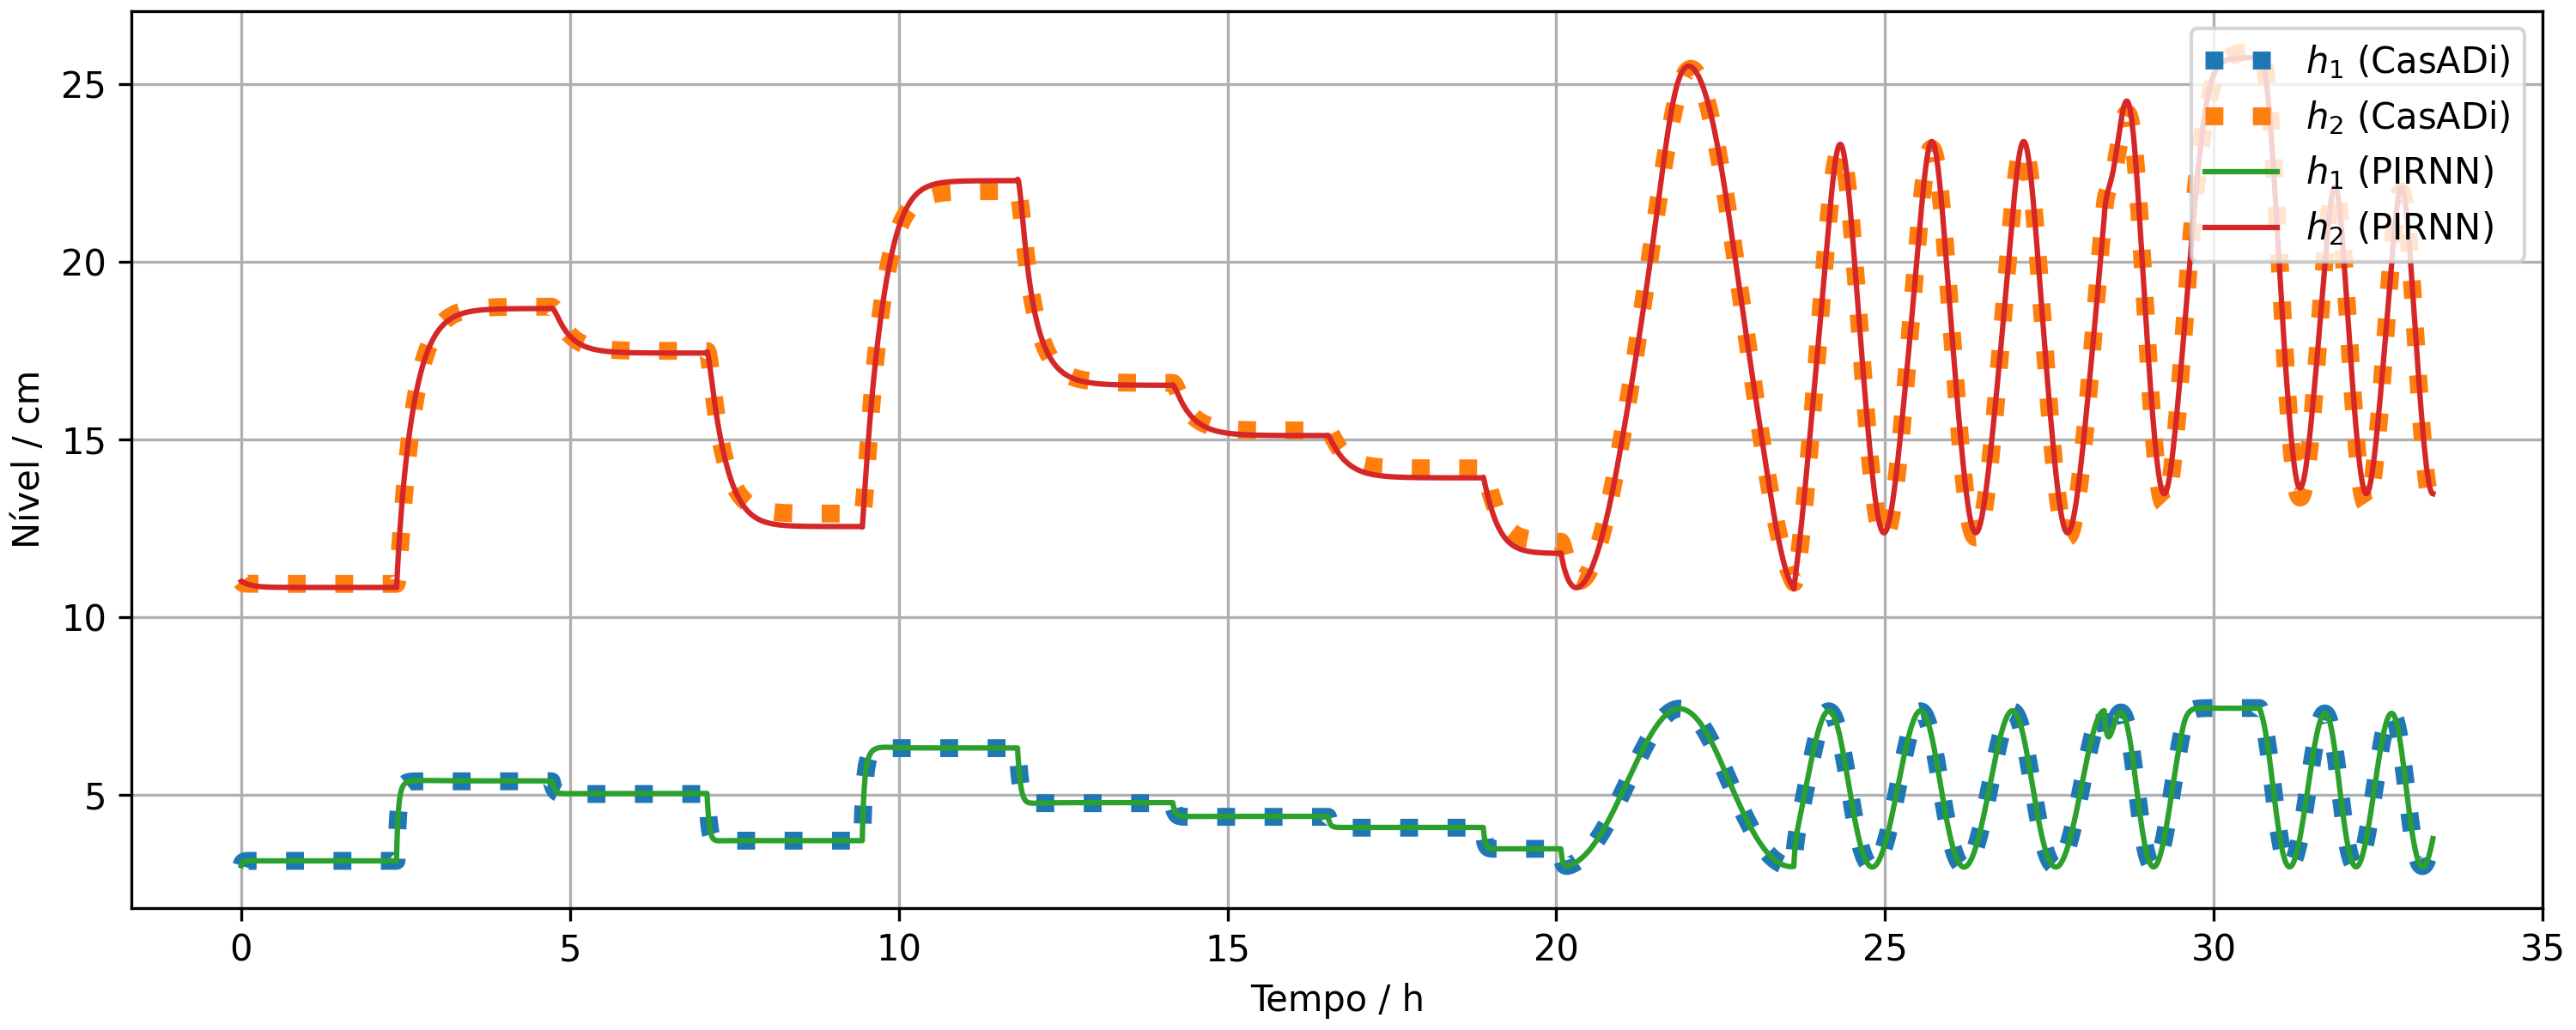
\includegraphics[width=0.9\textwidth]{pirnn-test-big.png}
    \caption{Comparação entre as previsões da PIRNN e o método numérico (RK)}
  \end{figure}
\end{frame}

\begin{frame}{Comparação de Tempos de Execução}
  \begin{figure}
    \centering
    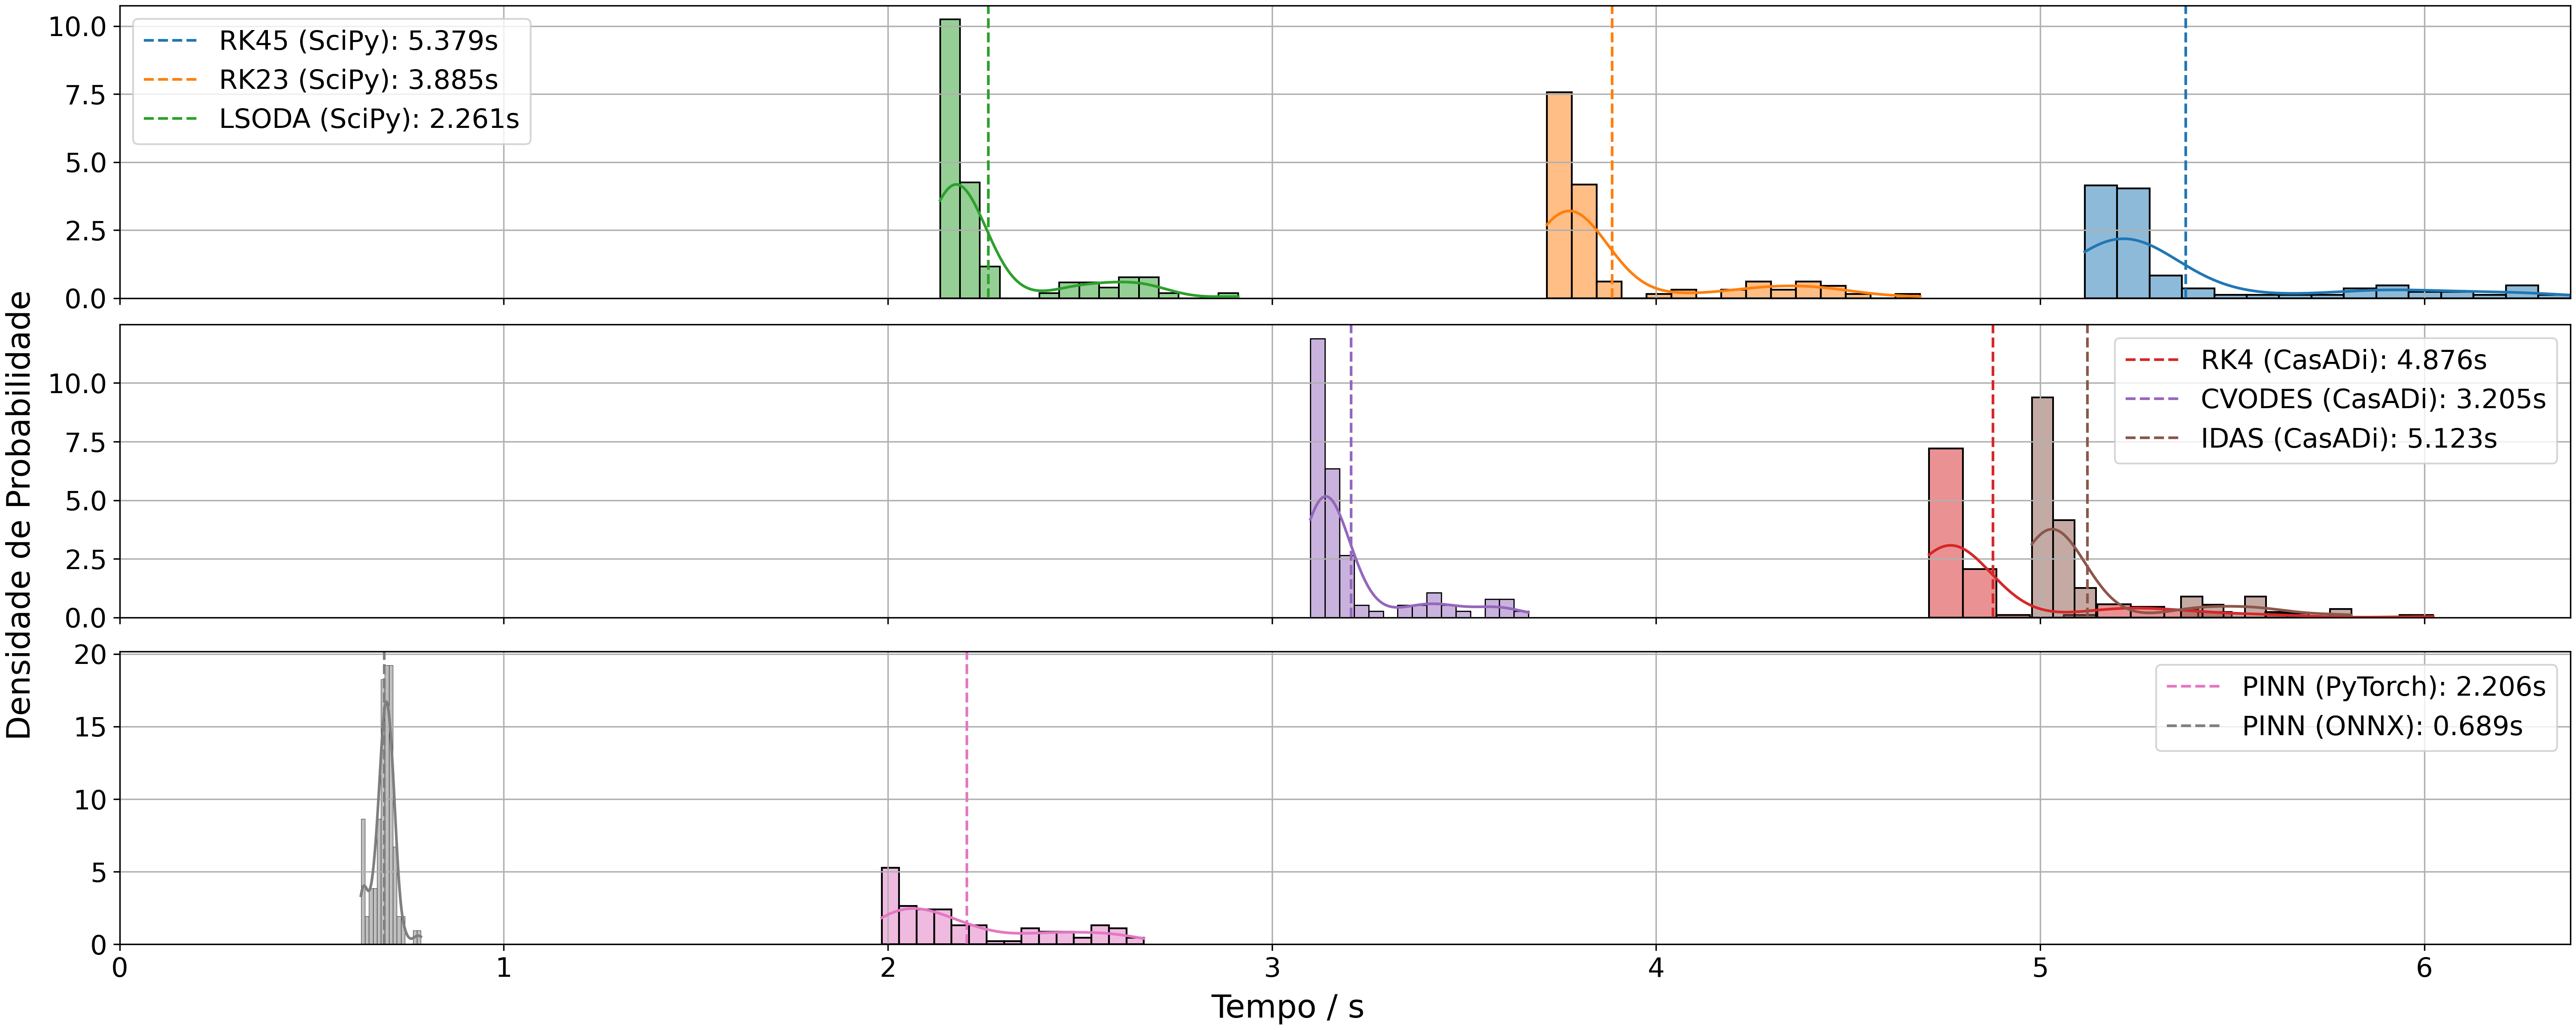
\includegraphics[width=0.85\textwidth]{pirnn-benchmark.png}
    \caption{Densidade de probabilidade dos tempos de execução dos métodos avaliados. Cada método foi executado 100 vezes; as linhas tracejadas indicam os tempos médios.}
  \end{figure}
\end{frame}

\begin{frame}{Por que o ONNX Runtime é tão rápido?}
  \begin{columns}
    \column{0.5\textwidth}
    O ONNX Runtime é focado em desempenho de inferência e possui uma série de otimizações:
    \begin{itemize}
      \item ``constant folding'';
      \item ``redundant node eliminations'';
      \item ``node fusions''.
    \end{itemize}

    \column{0.5\textwidth}
    \begin{figure}
      \centering
      \includegraphics[width=4cm, keepaspectratio]{onnx.png}
      \caption{Logo do ONNX Runtime. Fonte: onnxruntime.ai (2017)}
    \end{figure}

  \end{columns}
\end{frame}